% Front cover page
\newcommand{\DndCoverSplotch}{img/cover-splotch}
\newcommand{\DndCoverSplotchText}{Splotch Text}
\newcommand{\DndSubcoverSubtitle}{Subcover Subtitle}
\newcommand{\DndTitle}{Cover Title}
\newcommand{\DndSubtitle}{Cover Subtitle}
\newcommand{\DndTagline}{Cover Tagline}

\newlength\mylength
\renewcommand\cftchappresnum{\chaptername~}
\renewcommand\cftchapaftersnum{:}
\settowidth\mylength{\cftchappresnum\cftchapaftersnum\quad}
\addtolength\cftchapnumwidth{\mylength}

% StrokeColor, FillColor, StrokeWidth, Text
\newcommand*{\fillstroke}[4]{%
	% this is black magic
	% ref: http://tex.stackexchange.com/a/225639/125447
	% Tr: rendering mode (0=Fill, 1=Stroke, 2=FillThenStroke)
	% w: stroke width
	\special{pdf:bcolor #1 #2}%
	\special{pdf:literal direct #3 w 2 Tr}%
	#4%
	% ref: http://project.ktug.org/dvipdfmx/doc/tug2005.pdf
	\special{pdf:ecolor}%
	\special{pdf:literal direct 0 Tr}%
}

\newlength{\ox}
\newlength{\oy}

\ifdefined\isdraft
	\setlength{\ox}{.5\stockwidth-.5\paperwidth}
	\setlength{\oy}{.5\stockheight-.5\paperheight}
	\settrims{\oy}{\ox}
\else
	\setlength{\ox}{0pt}
	\setlength{\oy}{0pt}
\fi

\NewEnviron{tb*}[3]{%
	\begin{textblock*}{#1}(\ox+#2,\oy+#3)\BODY\end{textblock*}%
}

\NewEnviron{rtb*}[3]{%
	\TPoptions{absolute=false}%
	\begin{textblock*}{#1}(#2,#3)\BODY\end{textblock*}%
	\TPoptions{absolute=true}%
}

\newcommand*{\CoverPageBackground}[1]{
	\tikz[remember picture,overlay]
	\node[opacity=1,inner sep=0pt] at (current page.center)
	{
		\includegraphics[width=\paperwidth, keepaspectratio]{#1}
	};
}

\newcommand{\DndMakeCover}{
	\onecolumn%
	\thispagestyle{empty}%
	\CoverPageBackground{img/cover}
	\begin{center}%
		\vspace*{-15mm}
\includegraphics[width=3cm]{img/cover-logo-homebrewery}\\*\vspace*{15mm}%

		\fontsize{48pt}{48pt}\selectfont%
		\textpdfrender{
			TextRenderingMode=FillStroke,
			LineWidth=1.5pt,
			FillColor=CharFillColor,
		}{\nodesto{\DndTitle}}\\*%
		\normalfont\normalsize
\includegraphics[width=.5\paperwidth]{img/separator}\\%
		\fontsize{48pt}{48pt}\selectfont%
		%\textpdfrender{
		%	TextRenderingMode=FillStroke,
		%	LineWidth=1.5pt,
		%	FillColor=CharFillColor,
		%}{\DndSubtitle}\\*%
	\end{center}%
	\begin{figure*}[!b]
		\normalfont\normalsize
		\begin{adjustwidth}{-20mm}{0mm}
			\color{white}
			%\vspace*{17.0cm}
			\begin{overpic}[percent,unit=1mm,scale=.31]{\DndCoverSplotch}
				\put(12,5){\huge\texgyrebonum{\DndCoverSplotchText}}
			\end{overpic}
		\end{adjustwidth}
		\begin{center}%
			\normalfont\normalsize
			\LARGE\vfill%
			%https://tex.stackexchange.com/questions/25221/outlined-characters/108348#108348
			\textpdfrender{
				TextRenderingMode=FillStroke,
				LineWidth=0.5pt,
				FillColor=CharFillColor,
			}{\alegreyasansbold{\DndTagline}}\\*%
			% XXX: font doesn't look right
		\end{center}%
	\end{figure*}
	\pdfbookmark[0]{Front Cover}{Front Cover}
	\normalfont\normalsize
	\clearpage%
	\twocolumn%
}

\newcommand{\DndBlankPage}{%
	\onecolumn%
	\thispagestyle{empty}%
	\begin{center}%
		\LARGE\vfill%
	\end{center}%
	\normalfont\normalsize
	\clearpage%
	\twocolumn%
}

\newcommand{\DndMakeSubcover}{%
	\onecolumn%
	\thispagestyle{empty}%
	\begin{center}%
		\fontsize{48pt}{48pt}\selectfont%
		\nodesto{\bfseries{\DndTitle}}\\*%
		\normalfont\normalsize
\includegraphics[width=.5\paperwidth]{img/separator}\\%
		\fontsize{48pt}{48pt}\selectfont%
		%\DndSubtitle\\*%
		\normalfont\normalsize
		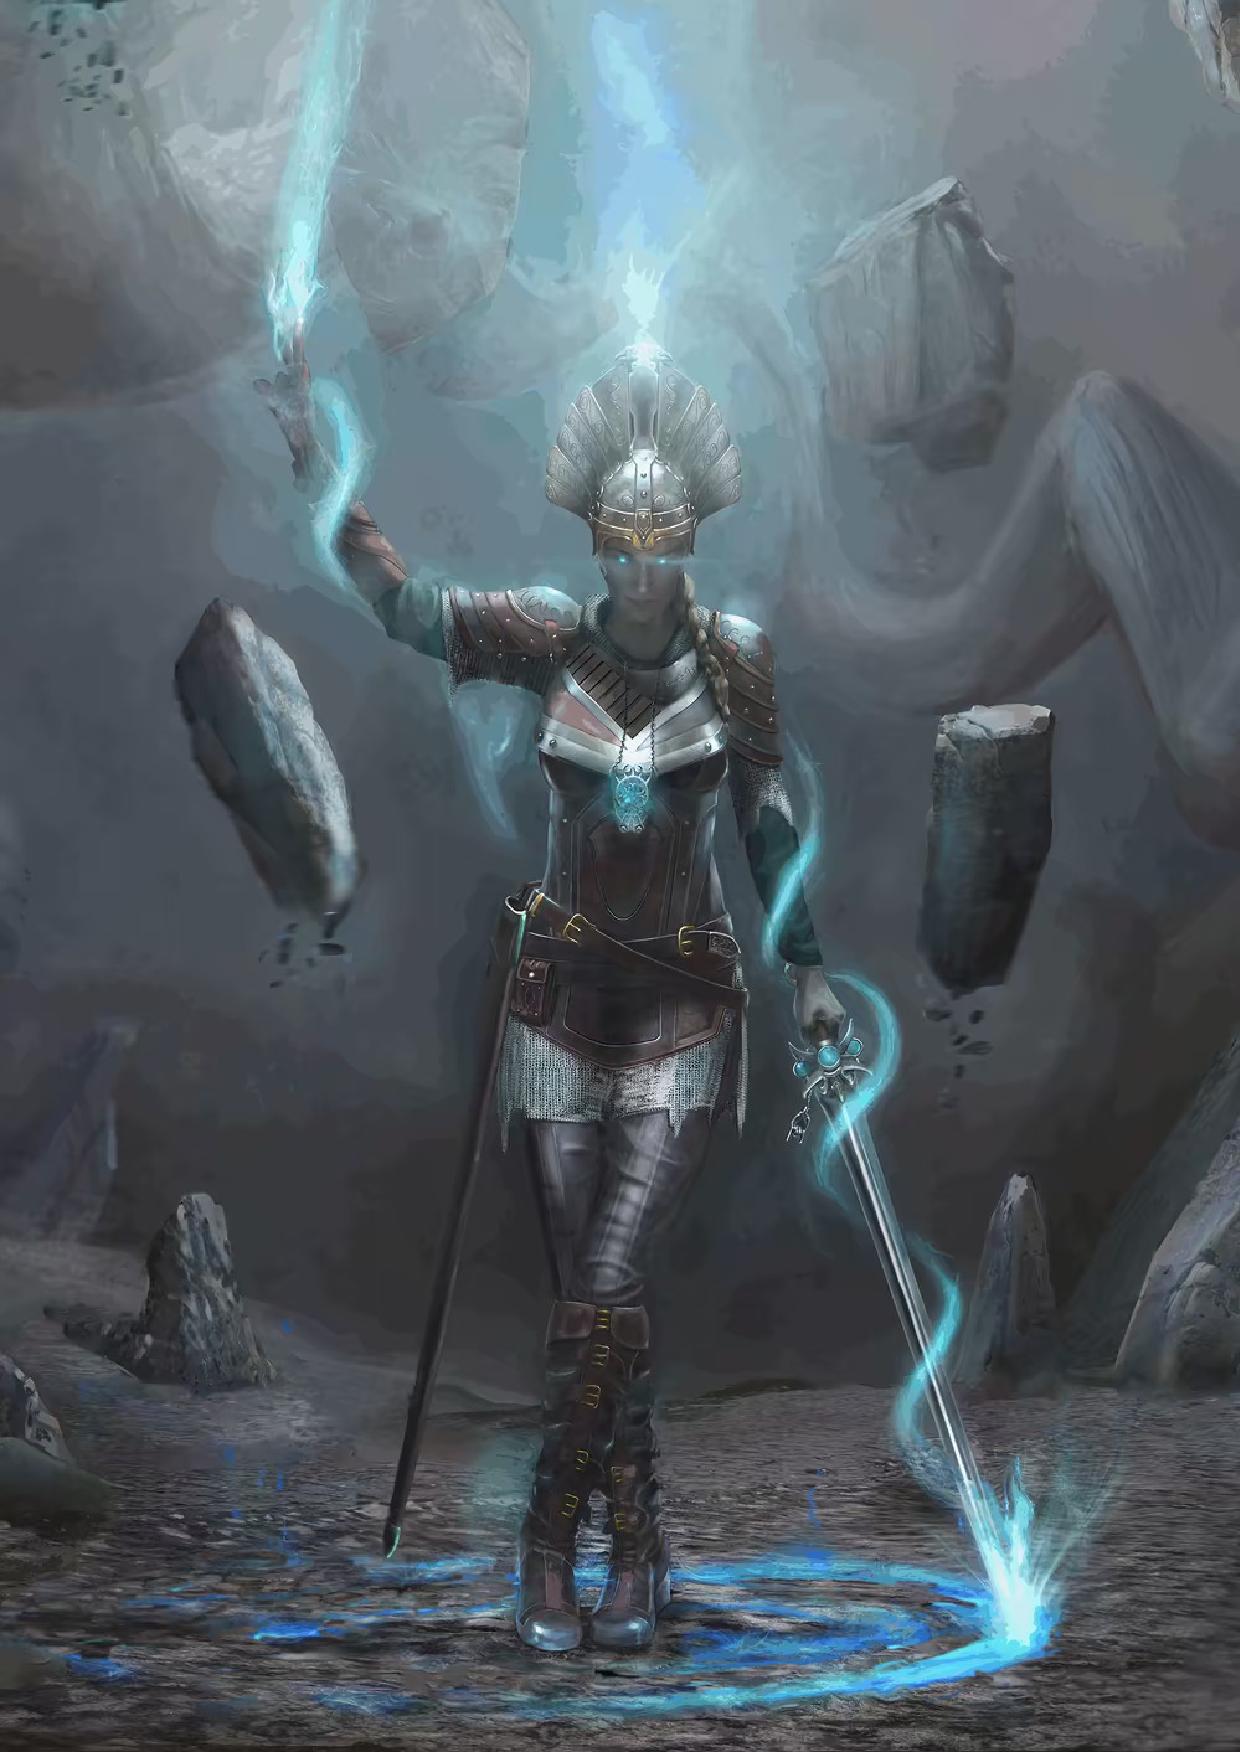
\includegraphics[width=10cm,keepaspectratio]{img/subcover}\\
		\LARGE\vfill%
		%\alegreyasansbold{\DndSubcoverSubtitle}\\%
		\vspace*{-15mm}
\includegraphics[width=3cm]{img/cover-logo-homebrewery}\\*\vspace*{15mm}%
	\end{center}%
	\normalfont\normalsize
	\clearpage%
	\twocolumn%
}

% Back cover page
\newcommand{\DndBackcover}{img/cover}
\newcommand{\DndBackcoverHeader}{Header.}
\newcommand{\DndBackcoverClose}{Closing sentence.}
\newcommand{\DndBackcoverDescription}{Description.}
\newcommand{\DndBackcoverLink}{\url{https://example.org}}
\newcommand{\DndBackcoverLogo}{img/dnd-logo-homebrewery}

\newcommand{\DndMakeBackcover}{%
	\onecolumn%
	\thispagestyle{empty}%
	\begin{tikzpicture}[remember picture,overlay]%
		\node[opacity=1, inner sep=0pt, anchor=east] (DndBackcover) at (current page.east)
		{
			
\includegraphics[width=\paperwidth,height=\paperheight]{img/backcoverimage}
		};%
	\end{tikzpicture}

	\begin{tikzpicture}[remember picture,overlay]%
		\node[opacity=1, inner sep=0pt, anchor=west] (Backcover) at (current page.west)
		{
			
\includegraphics[width=0.55\paperwidth,height=\paperheight]{img/backcover}
		};%
	\end{tikzpicture}

	\begin{multicols*}{2}
		\vspace*{2mm}
		\begin{center}
			\definecolor{Backcoverheadercolor}{HTML}{ff2a1a}
			\fontsize{36pt}{36pt}\selectfont%
			\textpdfrender{
				TextRenderingMode=FillStroke,
				LineWidth=0.5pt,
				FillColor=CharFillColor,
			}{\nodesto{\textcolor{Backcoverheadercolor}{\DndBackcoverHeader}}}\\*%
		\end{center}
		\begin{flushleft}%
			\normalfont\normalsize
			\color{white}
			\fontsize{12pt}{12pt}\selectfont%
			\textpdfrender{
				TextRenderingMode=FillStroke,
				LineWidth=0.5pt,
				FillColor=CharFillColor,
			}{\alegreyasansbold{\DndBackcoverDescription}}\\*%
		\end{flushleft}%
		\begin{center}%
			
\includegraphics[width=.25\paperwidth]{img/separator}\\%
			\vspace*{2mm}
			\normalfont\normalsize
			\color{white}
			\fontsize{12pt}{12pt}\selectfont%
			\textpdfrender{
				TextRenderingMode=FillStroke,
				LineWidth=0.5pt,
				FillColor=CharFillColor,
			}{\alegreyasans{\DndBackcoverClose}}\\*%
			\LARGE\vfill%
			\includegraphics[width=3cm]{\DndBackcoverLogo} \\%
			\fillstroke{[1]}{[0]}{.5}{\textbf{\DndBackcoverLink}}%
		\end{center}%
	\end{multicols*}
	\normalfont\normalsize
	\pdfbookmark[0]{Back Cover}{Back Cover}
	\clearpage%
}

\usetikzlibrary{intersections}
\tcbuselibrary{skins}

% Code from Loop Space: <https://tex.stackexchange.com/a/26386/73317>
\makeatletter
\tikzset{
  use path for main/.code={%
    \tikz@addmode{%
      \expandafter\pgfsyssoftpath@setcurrentpath\csname tikz@intersect@path@name@#1\endcsname
    }%
  },
  use path for actions/.code={%
    \expandafter\def\expandafter\tikz@preactions\expandafter{\tikz@preactions\expandafter\let\expandafter\tikz@actions@path\csname tikz@intersect@path@name@#1\endcsname}%
  },
  use path/.style={%
    use path for main=#1,
    use path for actions=#1,
  }
}
\makeatother
% End of the code from Loop Space

\colorlet{ornamentedFrameInner}{black}
\definecolor{ornamentedFrameOuter}{HTML}{deb400}

\tikzset{ornamented frame inner/.style={color=ornamentedFrameInner,
                                        line width=2pt},
         ornamented frame outer/.style={color=ornamentedFrameOuter,
                                        line width=3pt}}

\tcbsubskin{ornamented}{empty}{
  skin first=ornamented, skin middle=ornamented, skin last=ornamented,
  title engine=standard,
  frame code={
    % Account for the line widths in order not to draw beyond the bounding
    % box---except for a few very small details for which this is intentional.
    \coordinate (north west) at ([shift={(1.5pt,-1.5pt)}]frame.north west);
    \coordinate (north east) at ([shift={(-1.5pt,-1.5pt)}]frame.north east);
    \coordinate (south east) at ([shift={(-1.5pt,1.5pt)}]frame.south east);
    \coordinate (south west) at ([shift={(1.5pt,1.5pt)}]frame.south west);
    %
    \foreach \xoffset/\point in {34pt/north west, -34pt/north east,
                                  34pt/south west, -34pt/south east} {
      \fill[color=ornamentedFrameOuter]
        ([xshift=\xoffset]\point) circle[radius=2.5pt];
    }
    %
    \path[name path=ornament 1]
                                 ([yshift=-4pt]north west)
      [rounded corners=0.5pt] -- ++(23pt,0)
      [rounded corners=2pt]   -- ++(3pt,-4pt)
                              -- ([shift={(-26pt,-8pt)}]north east)
      [rounded corners=0.5pt] -- ++(3pt,4pt)
      [rounded corners=4pt]   -- ([yshift=-4pt]north east)
                              -- ([yshift=4pt]south east)
      [rounded corners=0.5pt] -- ++(-23pt,0)
      [rounded corners=2pt]   -- ++(-3pt,4pt)
                              -- ([shift={(26pt,8pt)}]south west)
      [rounded corners=0.5pt] -- ++(-3pt,-4pt)
      [rounded corners=4pt]   -- ([yshift=4pt]south west)
                              -- cycle;
    %
    \path[rounded corners=0.5pt, name path=ornament 2]
                                 ([yshift=-20pt]north west)
                              -- ++(-4pt,3pt)
                              -- ++(0,4pt)
               to[out=0, in=-90] ([shift={(8pt,0pt)}]north west)
                              -- ([shift={(34pt,0pt)}]north west)
                              -- ([shift={(-8pt,0pt)}]north east)
             to[out=-90, in=180] ([shift={(4pt,-13pt)}]north east)
                              -- ++(0,-4pt)
                              -- ++(-4pt,-3pt)
                              -- ([yshift=20pt]south east)
                              -- ++(4pt,-3pt)
                              -- ++(0,-4pt)
              to[out=180, in=90] ([shift={(-8pt,0pt)}]south east)
                              -- ([shift={(8pt,0pt)}]south west)
                to[out=90, in=0] ([shift={(-4pt,13pt)}]south west)
                              -- ++(0,4pt)
                              -- ++(4pt,3pt)
                              -- cycle;
    %
    \draw[ornamented frame outer, use path=ornament 1];
    \draw[ornamented frame outer, use path=ornament 2];
    \draw[ornamented frame inner, use path=ornament 1];
    \draw[ornamented frame inner, use path=ornament 2];
    %
    \foreach \xoffset/\point in {34pt/north west, -34pt/north east,
                                 34pt/south west, -34pt/south east} {
      \fill[color=ornamentedFrameInner]
        ([xshift=\xoffset]\point) circle[radius=2pt];
    }
  }
}

% These parameters---especially those related to geometry---are better located
% here in a style than in the subskin definition (see the Subskins section of
% the tcolorbox manual).
\tcbset{ornamented/.style={skin=ornamented, toptitle=14.5pt, bottom=9.5pt,
                           coltitle=black}
}

% Define the 'ornamentedbox' environment
\newtcolorbox{ornamentedbox}[1][]{ornamented, fonttitle=\scshape, #1}

% Convenient style to use with a tcolorbox preceded by text (or anything),
% when one wants to prevent any page break before the tcolorbox.
\tcbset{skip and no break/.style={
  before={\par\nopagebreak\vspace{2ex}\noindent}}
}

% Style suitable for an “on line” (in the middle of a paragraph)
% 'ornamentedbox'.
\tcbset{my on line/.style={
  capture=hbox, tcbox raise base, top=14pt, bottom=14pt,
  before={\kern 5pt}, after={\kern 5pt}}
}
